\documentclass[a4paper, 10pt]{article}
\usepackage[margin = 1in]{geometry}
\usepackage{amsmath}
\usepackage{tabularx}
\usepackage{framed}
\setlength{\parindent}{0em}
\newcolumntype{L}{>{\arraybackslash}m{10cm}}
\newcolumntype{T}{>{\arraybackslash}m{6cm}}
\usepackage{graphicx}
\usepackage{pdfpages}

\begin{document}

\section*{Topic 13 - Electric Fields}
\section{Electric Force}

\subsection{Coulomb's law}
\begin{framed}
   \textbf{Coulomb's law} states that the force between two point charges is proportional to the product of the charges and inversely proportional to the square of the distance between them
   \[
      F \propto \frac{Qq}{r^2}
   \]

   For two charges $Q$ and $q$ separated by a distance $r$,
   \[
   F = \frac{1}{4 \pi \varepsilon_0}\frac{Qq}{r^2}
   \]
   where $\varepsilon = 8.85 \times 10^{-12} Fm^{-1}$  \\
 
   Electric force is a \textbf{vector} quantity
\end{framed}	

\section{Electrical field strength}

\subsection{Eletric field}
\begin{framed}
   An \textbf{electric field} is a region of space in which a charge placed in that region experiences an electric force
\end{framed}	

\subsection{Electric field lines}
\begin{itemize}
   \item the \textbf{direction of an electric field line} indicates the direction of the electric force acting on a \textbf{small positive test charge} placed at that point. The direction of the electric field strength is tangent to the electric field lines at any point
   \item the \textbf{density of field lines} indicates the relative magnitude of electric field strength
   \item Electric field lines \textbf{originate from positive charges} and \textbf{terminate on negative charges}
\end{itemize}	

\textbf{Note that for a conductor}, placed inside an electric field, free electrons in an isolated solid or hollow conductor will redistribute until electrostatic equilibrium is achieved, hence
\begin{itemize}
   \item no electric field within conductor
   \item electric field lines must start or en dat the surface of the conductor, and be perpendicular to the surface of the conductor
   \item \textbf{potential within the conductor is constant}: there is no potential difference between any points
\end{itemize}	

\subsection{Electric field strength, $E$}
\begin{framed}
   the \textbf{electric field strength} at a point is defined as the electric force exerted per unit \textbf{positive} test charge 
   \[
   E = \frac{F}{q}
   \]
   The electric field strength due to charge $Q$ at a distance $r$ is 
   \[
      E = \frac{1}{4 \pi\varepsilon_0} \frac{Q}{r^2} 
   \]
   
   Electric field strength is a \textbf{vector} quantity
\end{framed}	

\subsection{Electric field strength of a charged conducting sphere}
For a \textbf{charged hollow or solid conducting sphere}, 
\begin{itemize}
   \item outside the sphere, electric field behaves as if all its charges are concentrated at its center, i.e. assumed to be point charge
   \item inside the sphere, $E = 0$  because all the charges are uniformly distributed on the surface of the sphere. The potential within the sphere is the same as that on the surface of the sphere
\end{itemize}	


\section{Electric Potential and Electric potential energy}


\begin{framed}
   The \textbf{electrical potential} at a point in an electric field is defined as the work done \textbf{per unit positive test charge} by an external force in bringing a small test charge from infinity to that point
   \[
   V = \frac{W}{q}
   \]

   The electric potential $V$  at a distance $r$ away from charge $Q$ is 
   \[
      V = \frac{W}{q} = \frac{1}{q} \int_{\infty}^{r} F_{ext}dr = \frac{1}{4\pi\varepsilon_0} \frac{Q}{r}
   \]

   The electrical potential at a point due to multiple charges can be found by \textbf{adding} the individual potentials at that point due to each charge
\end{framed}	

\begin{framed}
   The \textbf{electrical potential energy} of a charge at a point in an electric field is definend as the work done by an external force in bringing the charge from infinity to that point
   \[
   U = W = qV
   \]
   Hence, the electrical potential energy of a system of two point charges separated by r is
   \[
      U = \frac{1}{4\pi\varepsilon_0} \frac{Qq}{r}
   \]
\end{framed}	

\subsection{Electron volt $eV$ }
\begin{framed}
   The \textbf{electron-volt} is the energy gained by an electron when it is accelerated through a potential difference of one volt
   \[
      1\ eV = 1.60 \times 10^{-19} J
   \]
   
\end{framed}	

\subsection{Potential difference}
\[
   \Delta V = V_{final} - V_{initial}
\]

The work done and change in potential energy is 
\[
 W = \Delta U = q \Delta V
\]

\subsection{Relationships between $F,\ E,\ V,$ and $U$}
\begin{framed}
   \[
   E = - \frac{dV}{dr}
   \]
   The electric field strength at a point is numerically equal to the potential gradient at that point. \\

   Electric field strength points in the direction of decreasing potential
\end{framed}	

\begin{framed}
   \[
   F = - \frac{dU}{dr}
   \]
   The elctric force at a point is numerically equal to the potentialenergy gradient  \\
   The electric force points in the direction of decreasing potential
\end{framed}	


\section{Equipotential lines and surfaces}
\begin{itemize}
   \item equipotential lines are perpendicular to electric field lines
      \begin{itemize}
         \item hence there is no component of electric field strength acting on a charge that moves along an equipotential line
            \[
            W = 0
            \]
      \end{itemize}	
   \item movement along an equipotential line or surface requires no work since $\Delta V = 0$ 
      \[
         W = q\Delta V = q(0) = 0
      \]
   \item Dashed lines are used to represent equipotential lines

\end{itemize}	

\section{Uniform electric field}
\begin{itemize}
   \item the electric field strength at any point has the \textbf{same magnitude} and \textbf{direction}
   \item the electric field lines are \textbf{parallel} and \textbf{equally spaced} \\
\end{itemize}	
\begin{minipage}{0.5\textwidth}
\begin{center}
   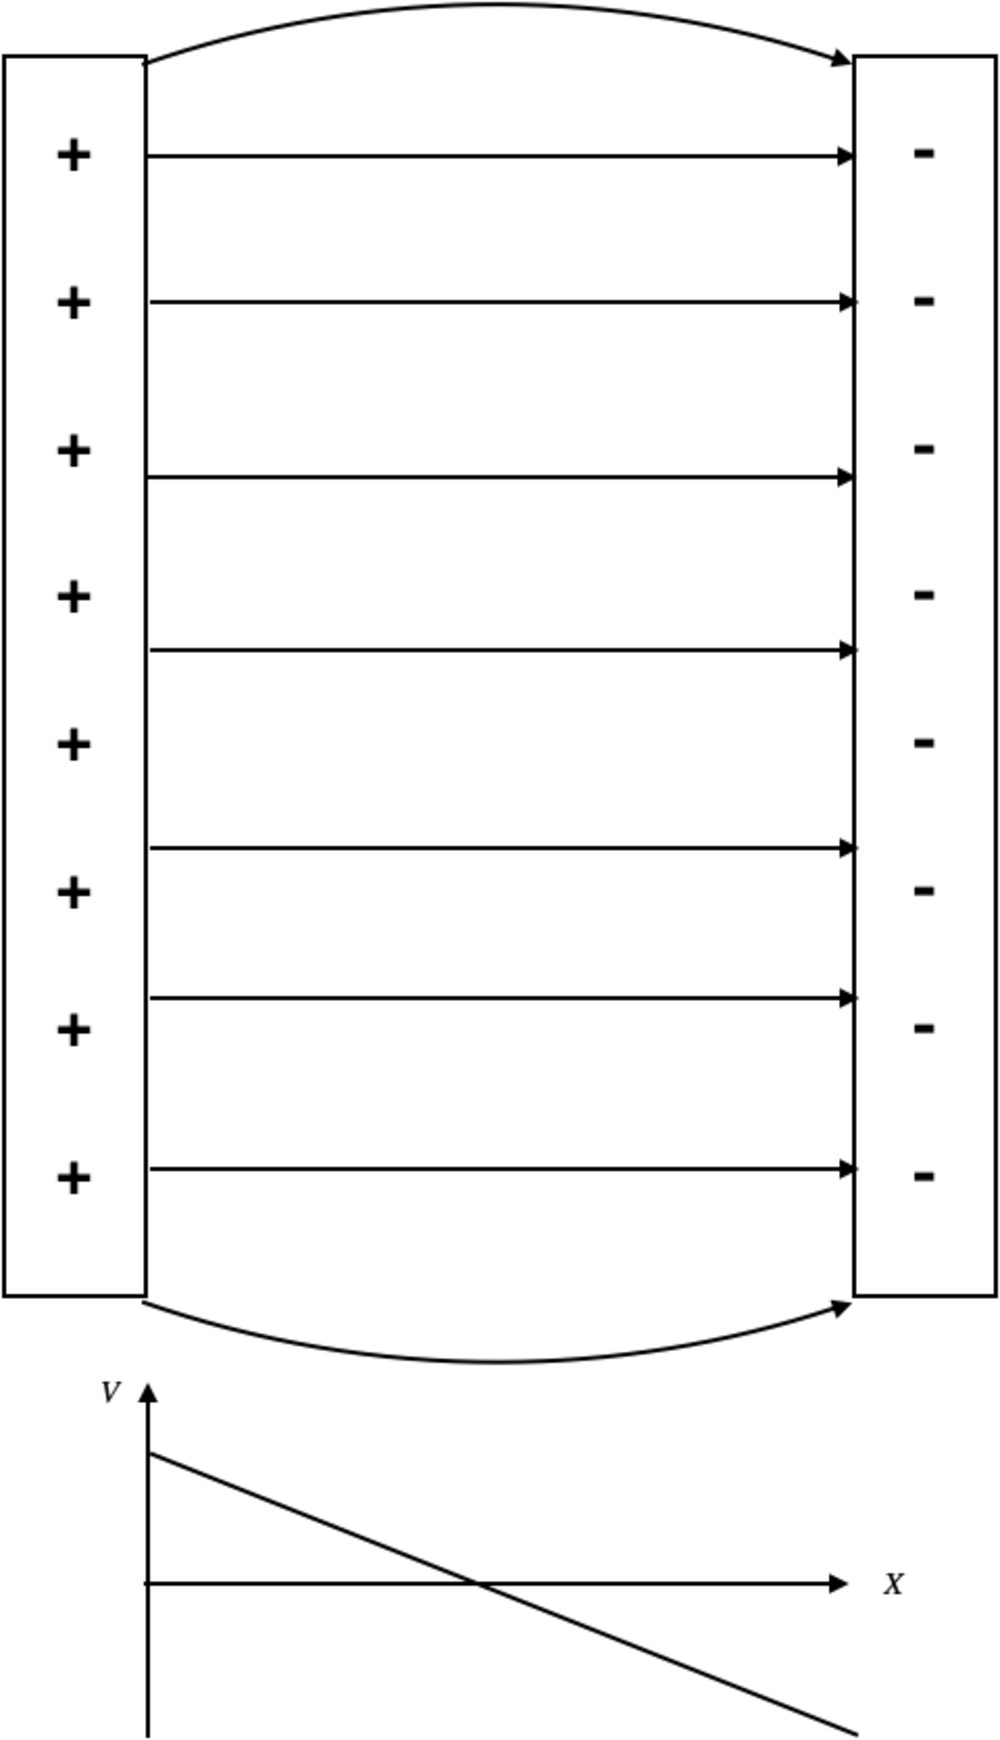
\includegraphics[trim = 50 50 50 50, width=3cm]{figures/1.pdf} 
\end{center}	
\end{minipage}	
\begin{minipage}{0.5\textwidth}
   Since electric field is uniform, the potential gradient at any points is constant
   \[
   \frac{dV}{dx} = -E
   \]

   Therefore, the magnitude of electric field strength is
   \[
   |E| = \left| \frac{\Delta V}{d} \right|
   \]

   The magnitude of $F$ on a charge q is
   \[
   F = qE
   \]
\end{minipage}	

\end{document}	
